\subsection{Effect of class weights}
\label{sec:effect_of_class_weights}
In the previous section we have speculated that the poor performance of the CNN on the test set is due to the unbalanced nature of the dataset. Among the most common techniques to deal with unbalanced datasets, using class weights is one of the simplest and most effective (unlike oversampling, it does not require additional computing power, nor does it cause loss of information in the dataset like undersampling). In this section we will evaluate the effect of different class weights on the validation performance of the CNNs.
\\ The experiments were carried out with the configurations transcribed in Tab. \ref{tab:class_weights}. In particular, observe that:
\begin{itemize}
    \item \textbf{W1} corresponds to the default configuration, i.e. no class weights;
    \item \textbf{W2} is computed automatically to balance the training set;
    \item \textbf{W3} is composed of the ratios between the number of samples in each class in the test set and in the training set;
    \item the remainder is chosen arbitrarily.
\end{itemize}

\begin{table}[ht]
    \centering
        \begin{tabular}{cccccc}
        \hline
        \textbf{Weights} & \textbf{Class 0} & \textbf{Class 1} & \textbf{Class 2} & \textbf{Class 3} & \textbf{Class 4} \\ \hline
        W1                     & 1.000            & 1.000            & 1.000            & 1.000            & 1.000            \\
        W2                     & 1.274            & 0.849            & 0.849            & 0.637            & 3.452            \\
        W3                     & 0.133            & 0.183            & 0.271            & 0.948            & 0.106            \\
        W4                     & 1.200            & 1.000            & 1.000            & 0.700            & 2.200            \\
        W5                     & 0.900            & 1.000            & 1.000            & 0.800            & 1.800            \\
        W6                     & 1.000            & 1.000            & 1.000            & 0.200            & 2.000            \\
        W7                     & 0.600            & 0.700            & 0.700            & 0.400            & 2.000            \\ \hline
        \end{tabular}
    \caption{Class weights used for the experiments.}
    \label{tab:class_weights}
\end{table}

\noindent As seen in Sec. \ref{sec:classification_scores}, evaluating the class-wise performance is as crucial as evaluating the overall one. For the latter we can use validation loss (do not forget that this is the metric monitored by the early stopping callback, hence we will necessarily look at the best one after epoch 20), while for the former we may use f1-score, which summarizes the precision and recall scores for each class. 

\noindent \\The plots in Fig. \ref{fig:weights_loss} and \ref{fig:weights_f1} show the outcomes of the experiments. Observe that:
\begin{itemize}
    \item using no class weights (W1) is definitely better than using the ones computed automatically (W2), since the validation set unbalance is even more severe than the training set one;
    \item W3 is the best configuration in terms of validation loss since it is taylored on the test set, but it scores 0 in terms of f1-score for class 4 for both models, thus it would not be a good choice for driving the race car;
    \item W6 penalizes excessively the majority class 3 and (as a consequence) the validation loss skyrockets, thus it is the worst configuration;
    \item finally, the two models score significantly different f1-scores with the same weights - especially using W3 and W6 - but the validation losses are very similar.
\end{itemize}

\begin{figure}[htbp]
    \centering
    \subfloat[Model 0.]{
        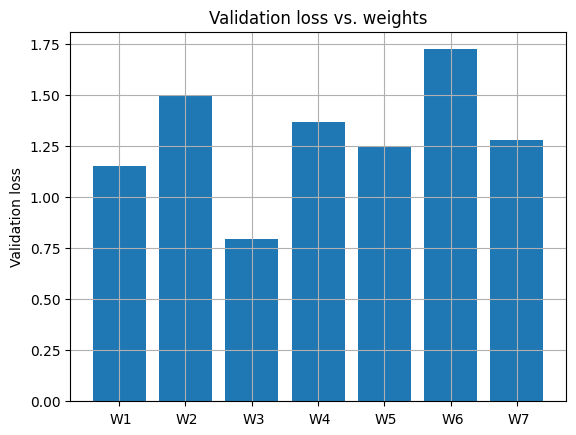
\includegraphics[width=0.4\textwidth]{figures/images/weights_loss_m0.png}
        \label{fig:weights_loss_m0}
    }
    \subfloat[Model 1.]{
        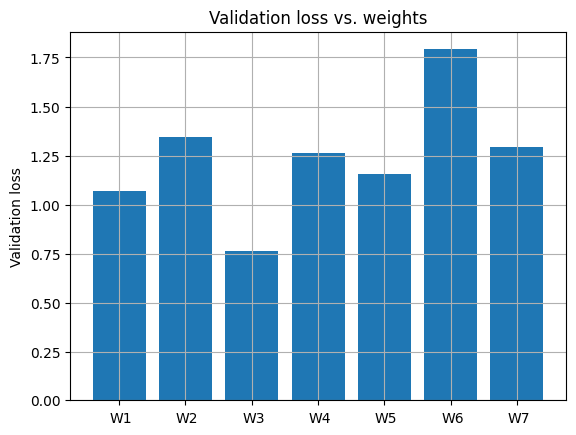
\includegraphics[width=0.4\textwidth]{figures/images/weights_loss_m1.png}
        \label{fig:weights_loss_m1}
    }
    \caption{Effect of different class weights on the validation loss.}
    \label{fig:weights_loss}
\end{figure}
\begin{figure}[htbp]
    \centering
    \subfloat[Model 0.]{
        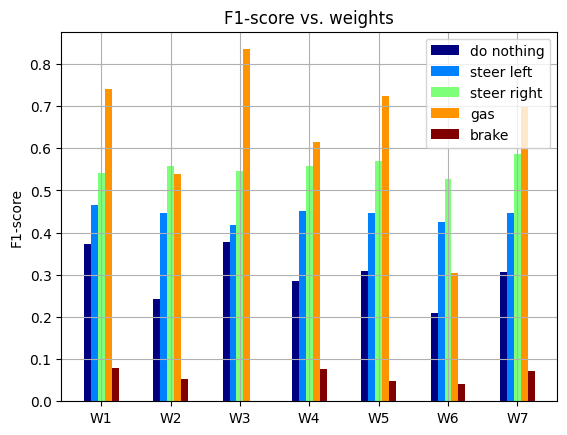
\includegraphics[width=0.4\textwidth]{figures/images/weights_f1_m0.png}
        \label{fig:weights_f1_m0}
    }
    \subfloat[Model 1.]{
        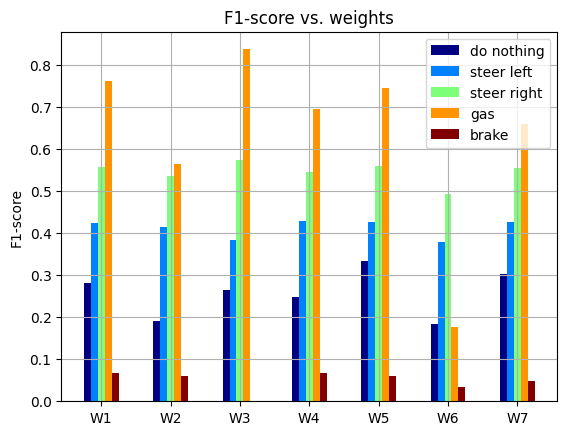
\includegraphics[width=0.4\textwidth]{figures/images/weights_f1_m1.png}
        \label{fig:weights_f1_m1}
    }
    \caption{Effect of different class weights on the class-wise f1-score.}
    \label{fig:weights_f1}
\end{figure}

\noindent The final choice of weights is W4, which is the one that provides the best trade-off between validation loss, f1-scores and driving capabilities (see App. \ref{sec:driving_race_car}). As a matter of fact, the results reported in the previous sections were obtained with this configuration.